\documentclass[a4paper,11pt]{report}
\usepackage[T1]{fontenc}
\usepackage[utf8]{inputenc}
\usepackage{lmodern}
\usepackage[italian]{babel}
\usepackage{graphicx}
\usepackage{tikz}
\usepackage{pgfplots}
  \usepgflibrary{arrows}
\usepackage{float}
\usepackage{amssymb,amsmath}

\title{Appunti del corso di Misure}
\author{Andrea Donati - AA 2018/19}
\begin{document}

\maketitle
\tableofcontents

\begin{abstract}
Appunti presi a lezione e trascritti in modo da essere human-readable, contrariamente alle slide fornite dal professore.
\end{abstract}
\newpage
\chapter{Metrologia e Sistema Internazionale}
\section{Definizioni Metrologiche}
Diamo una prima definizione di ciò che chiamiamo "misura".\\
\bf Misura \rm può essere:

\begin{itemize}
  \item un procedimento di misurazione, che porta all'assegnazione di un valore a una grandezza fisica detta misurando.
  \item risultato della misurazione, che deve essere espresso in una maniera tale da essere comprensibile in tutte le sue forme: valore numerico, unità di misura e \bf incertezza \rm associata alla misura. Oggi il risultato di una misurazione è convenientemente espresso in questo modo.
\end{itemize}

Una \bf Grandezza\rm: attributo di un fenomeno o di una sostanza distinguibile \it qualitativamente \rm e determinabile \it quantitativamente\rm. Un esempio di Grandezza può essere l'altezza di un edificio, la \bf massa \rm di un TIR, la velocità di un fluido. Al contrario non possiamo definire "grandezza" la bellezza, la felicità, il gusto di un cibo, dato che queste non sono distinguibili qualitativamente, nè determinabili quantitativamente.
\\

Il \bf Misurando\rm: è il modo in cui ci riferiamo alla grandezza sottoposta a misura.
\\ 

Le \bf Grandezze Omogenee\rm: sono grandezze della stessa natura, e che quindi sono direttamente confrontabili tra loro. Una fondamentale caratteristica delle "grandezze omogenee" è che esse si esprimono nella
\bf stessa unità di misura\rm.
\\

Un'ulteriore definizione di \bf Misura \rm si può dare anche con le grandezze omogenee: una misura è il confronto tra due grandezze omogenee, di cui una è presa come \it riferimento \rm o \it campione di misura\rm.
\\

Il \bf Valore \rm di una misura è il numero che esprime il rapporto con il riferimento.
\\

Il riferimento di una misura può essere manufatto (una spanna, un piede, una tazza, un peso campione), od assoluto (un giorno, un ciclo lunare, 1 decimetro cubo di $H_2O$, proprietà della materia che difficilmente variano a seconda di tempo e spazio).
\\

Possiamo a questo punto fare degli esempi di misure sulla base di ciò che abbiamo definito fin'ora. Posso ad esempio misurare la lunghezza del mio tavolo da cucina in spanne, cioè prendendo la mia spanna come \bf riferimento\rm. La misura del tavolo avrà come \bf valore \rm, ad esempio, 7 e come unità di misura la spanna; diremo quindi "7 spanne".

Questa misura ha sicuramente un riferimento di tipo manufatto.
\\

Un esempio di misura di tipo assoluto è la misurazione di un intervallo di tempo in giorni. Ad esempio: sono passati \it 3 giorni\rm. l'unità di misura in questo caso è chiaramente il giorno.
\section{Errori di Misura}
È importante realizzare che, purtroppo, \bf non esiste \rm alcuna \it misura esatta\rm. Ogni misura è affetta da diversi contributi di errore, che si trasformano in cause di incertezza, le quali sono riducibili attraverso l'ingegnerizzazione della misura, ma non sono mai eliminabili.

Le possibili cause di incertezza di una misura possono essere dovute ai \it riferimenti \rm presi (nel caso dell'esempio precedente della misura del tavolo da cucina "a spanne", il riferimento preso è soggetto a forti cause di incertezza dato che è impossibile replicare la propria spanna esattamente ogni volta): si possono avere scostamenti dalla definizione dell'unità di misura utilizzata oppure variabilità del riferimento.

Anche i dati di origine sono fonte di incertezza in una misura, perché possono essere incompleti o scorretti, specie se risultati di altre misure.

Vi è inoltre la relazione tra misurando e sistema di misura che può causare incertezza, con \bf effetti di carico \rm ed \bf errori di modello\rm. Spieghiamo questi due concetti con altrettanti esempi:

\begin{itemize}
  \item \bf Effetto di Carico \rm è quello che si verifica, ad esempio, quando andiamo ad effettuare la misura di una tensione in un punto di un circuito elettrico con un voltmetro. Se inseriamo il voltmetro in un qualsiasi punto del circuito, per misurare la tensione esso usa una resistenza interna, quindi la tensione che in realtà leggiamo dal voltmetro avrà anche il contributo (seppur minimo) della resistenza interna del voltmetro. Se il voltmetro è "scarso" il fenomeno sarà più compromettente per la misura.
  \item \bf Errore di Modello \rm si verifica nel caso di misure indirette, ed è causato dalla relazione funzionale che descrive una misura indiretta. Più il modello sarà raffinato e completo, meno la misura risentirà dell'errore di modello. Un esempio può essere il calcolo della potenza elettrica sviluppata in un resistore che in prima analisi può essere $R \times I^2 $, ma esitono formule molto più precise per calcolarla.
  \item \bf Parametri ambientali (grandezze d'influenza)\rm: fattori come temperatura, pressione, umidità, vibrazioni o presenza di campi elettro-magnetici influenzano una misura.
  \item \bf Interazione occhio-strumento\rm: causa errori di parallasse, interpolazione e media.
  \begin{itemize}
    \item Parallasse: interessa gli strumenti analogici, è dovuto al non parallelismo tra il piano "di visione", cioè il piano sul quale ci poniamo come osservatori e il piano della "lancetta", che deve essere spostata dal piano della scala per muoversi.
    \item Interpolazione: la risoluzione dello strumento è troppo bassa per apprezzare tutti i livelli del misurando. La lancetta si ferma in una posizione intermedia tra due "tacchette" (immaginiamo quella dell'1 e quella del 2) e per cercare di desumere la misura l'utilizzatore stima ad occhio quanto essa sia più vicina all'una od all'altra tacchetta.
    \item Media: come spesso accade in risposta ad un rumore variabile nel sistema, la lancetta dello strumento ha delle oscillazioni ipoteticamente attorno al valore "giusto" della misura, quindi si cerca di indovinare tale valore. Questo tipo di errore è presente anche negli strumenti digitali i quali, in condizioni \bf ripetute \rm (vedremo poi cosa significa), mostrano valori diversi oltre una certa cifra decimale. L'utilizzatore allora registra tali valori differenti e li media. Questo approccio introduce anche un \bf filtro\rm, perché oltre una certa cifra decimale l'utilizzatore filtra, appunto, i risultati, mediandoli.
  \end{itemize}
  \item \bf Zero (offset)\rm: pensiamo di avere sottomano una bilancia qualsiasi, in un ipotetico grafico che mostra la corrispondenza valori "reali" di massa - valori misurati di massa. È desiderabile avere tutti i punti che appartengono alla retta bisettrice del primo (e terzo) quadrante. A volte non è così, ma la retta "propria" della bilancia è traslata in verticale di una certa quantità (pur mantenendo la pendenza).
  
  Può capitare di incontrare bilance, ad esempio per la pesa dei TIR, che "a vuoto" segnano già 100 Kg.
  \item \bf guadagno/pendenza (gain/slope)\rm: sempre riferendoci alla retta del punto precedente, questo errore si verifica quando la retta "reale" si differenzia dalla retta "ideale" per pendenza, per cui l'errore sarà maggiore al crescere della massa che si vuole misurare.
  \item \bf non-linearità\rm: sul grafico vediamo la differenza tra la curva ideale, che è una retta, e la curva reale, che non è lineare ed ha la massima distanza dalla retta ideale per i punti estremi.
  \item \bf Isteresi\rm: errore proprio degli apparecchi per misurazione che hanno al loro interno giochi meccanici, in questo caso gli errori di misura crescono mano a mano che si pesa ogni volta una massa maggiore/minore.
\end{itemize}

\section{Altre Definizioni Metrologiche}
Le seguenti definizioni sono tratte dal VIM (\it Vocabolario Internazionale di Metrologia\rm).

\begin{itemize}
  \item \bf Accuratezza\rm
  \begin{itemize}
    \item di un Campione: scarto tra la grandezza realizzata con il campione e la definizione dell'unità.
    \item di una Misura: vicinanza del valore di misura alla miglior stima possibile per il misurando.
    \item di uno Strumento: stima dell'incertezza dello strumento o confronto con uno migliore.
  \end{itemize}
  L'accuratezza NON è da confondere con l'incertezza.
  \item \bf Risoluzione\rm: capacità di uno strumento/misura di risolvere stati (livelli) diversi del misurando. ATTENZIONE: la risoluzione di uno strumento NON è "la minima grandezza misurabile"!!! Ma è il minimo intervallo di valori che è possibile apprezzare con il dato strumento.
  
  La risoluzione può essere una caratteristica qualitativa (alta/bassa) oppure quantitativa (si indica il valore della minima variazione apprezzabile).
  
  \item \bf Sensibilità\rm: rapporto tra la variazione della grandezza (segnale) di uscita e la corrispondente variazione della grandezza (segnale) d'ingresso.
  
  La sensibilità NON è l'esatta variazione dell'uscita rispetto all'ingresso, ma il RAPPORTO tra la variazione dell'ingresso e la variazione dell'uscita. La sensibilità indica quindi quanto una misura può essere fedele in un dato intervallo di valori rispetto ad altri intervalli di valori. Può essere quindi rappresentata da una curva, di cui il tratto iniziale è il tratto a maggior sensibilità, mentre più ci si avvicina alla saturazione (muovendosi a destra sulla curva) più la sensibilità decresce (con enfasi sulla zona finale).
  
  \item \bf Incertezza\rm: stima, eseguita secondo procedimenti convenzionali, del nostro livello di \it NON \rm conoscenza del misurando.
  
  \item \bf Ripetibilità\rm: capacità di ottenere, per uno stesso misurando, valori di lettura vicini tra loro \bf nel breve periodo \rm "nelle stesse condizioni" (stesso procedimento di misura, operatore, luogo e condizioni ambientali\dots).
  
  La ripetitibilità implica anche, ad esempio, la non-deteriorazione del misurando. La ripetibilità è da intendere proprio come capacità di misurare più volte e \bf nelle stesse condizioni\rm.
  
  \item \bf Riproducibilità\rm: capacità di ottenere, per uno stesso misurando, risultati vicini tra loro "in diverse e specificate condizioni di misura".
  
  Nella caratteristica della riproducibilità si elimina il vincolo temporale che era invece presente nella ripetibilità.
  
  \item \bf Riferibilità\rm: proprietà di una misura di essere messa in relazione (i.e. riferita) con quella fornita da un campione riconosciuto.
  
  Ad esempio, se eseguo la misura di un resistore in Ohm attraverso un Ohmmetro di scarsa qualità e ottengo $1\ K\Omega$, posso riferire la misura appena fatta a quella di un Ohmmetro di qualità molto migliore, il quale mi darà un valore più preciso, ad esempio $800\ \Omega$. Anche la misura di questo Ohmmetro può essere riferita ad una più precisa, ad esempio quella di un ente nazionale di misurazione, il quale riferirà le proprie misure ad un ente internazionale, fino ad arrivare al riferimento con la definizione/un campione.
  
  Questa successione di riferimenti è detta "catena di riferibilità", ed è abbastanza importante avere una catena di riferibilità corposa, piuttosto che averne una interrotta dopo un riferimento, perché significa che la mia misura non può essere molto confrontabile con altre più precise.
  
    \item \bf Stabilità\rm: capacità di ottenere, per uno stesso misurando, valori di lettura vicini tra loro in un intervallo di tempo ben definito e chiaramente specificato (con stesso procedimento di misura, operatore, luogo, e condizioni ambientali).
    
    Come la riproducibilità, ma durante il collezionamento delle misurazioni è necessario \bf specificare \rm l'orario in cui esse sono state prese.
  
\end{itemize}
\newpage
\section{Il Sistema Internazionale}

Le note storiche sono facilmente reperibili sia on-line sia dai lucidi del professore, quindi sono state trascurate durante la stesura degli appunti.
\begin{figure}[H]
  \begin{center}
    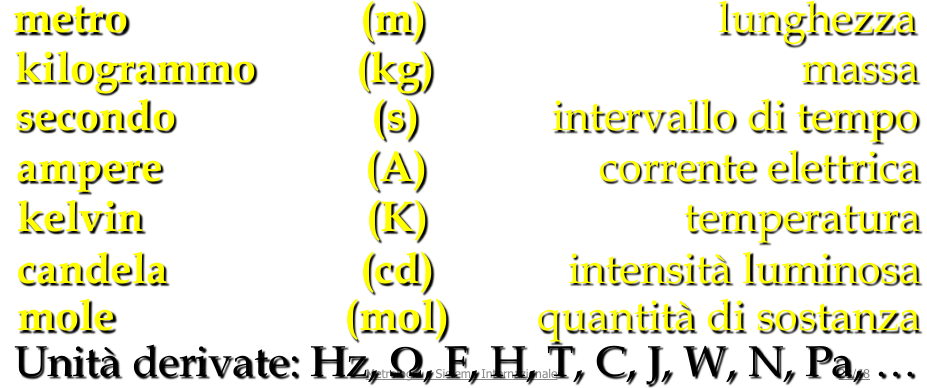
\includegraphics[
        width=12cm,
        height=6cm,
        keepaspectratio,
    ]{images/unitafondamentali.png}
    \caption{Le unità fondamentali del Sistema Internazionale.}
  \end{center}
\end{figure}
Il Sistema Internazionale è un \bf Sistema Coerente \rm in quanto tutte le sue unità derivate (qualunque grandezza G) si ricavano come prodotti e rapporti delle 7 unità di base, senza introdurre fattori moltiplicativi (come  $\pi,e,5\dots$).\\
Possiamo scrivere quindi che, indicando con "$dim(G)$" l'unità derivata dalle unità base SI: $$ dim(G) = L^\alpha M^\beta T^\gamma I^\delta \theta ^\varepsilon J^\eta N^\zeta  $$

Avendo:
\begin{itemize}
  \item L : Lunghezza (metro)
  \item M : Massa (kilogrammo)
  \item T : Intervallo di Tempo (secondo)
  \item I : Intensità di Corrrente (Ampere)
  \item $\theta$ : Temperatura (Kelvin)
  \item J : Intensità Luminosa (candela)
  \item N : Quantità di Sostanza (mole)
\end{itemize}

ognuno con il proprio esponente. Naturalmente, se la specifica unità base non compare nelle unità che compongono quella derivata, avrà esponente pari a $0$.
\\


Il Sistema Internazionale è anche un sistema completo? Tutte le unità di misura esistenti possono essere espresse attraverso le unità di base? Se così non fosse, sarebbe necessario aggiungere qualche unità a quelle del sistema internazionale.\\

Un'altra caratteristica importante del Sistema Internazionale è che le unità di base sono tra di loro dimensionalmente indipendenti, ma non logicamente indipendenti (e.g. il metro "dipende dal secondo").\\

Inoltre, nel S.I. esiste una sola unità di misura per ciascuna grandezza fisica, che è la corretta unità di misura di base o derivata da quelle di base. Ed è anche importante menzionare che attraverso uno qualsiasi dei \bf prefissi decimali approvati\rm, detti prefissi SI, può essere usato per costruire multipli e sottomultipli decimali delle unità di misura SI. Anche se sembra una caratteristica abbastanza naturale, esistono dei sistemi di misura che non la rispettano, ad esempio il sistema imperiale di misurazione delle distanze: la \it yard \rm non corrisponde a $1\ K\ inches$.

\subsection{Definzioni Assolute e Definizioni con Campioni Manufatti}
Nel Sistema Internazionale (ad oggi: settembre 2018), esistono ancora unità base definite attraverso dei campioni di riferimento, ad esempio il kilogrammo. Ebbene queste definzioni sono in un certo qual modo peggiori rispetto a quelle deifinite in modo assoluto, perché compromettendo il campione (ammettendo che esso sia unico, cosa che per fortuna non è - ne esistono diversi altri molto simili), si modificano virtualmente tutte le misure fatte da quel momento in poi. Un classico esempio espresso informalmente potrebbe essere "se qualcuno stanotte scambia il campione del kilogrammo, domani potremmo pesare tutti due etti in meno".

Le definizioni assolute invece sono "un'altra storia", perché esse sono realizzate attraverso costanti universali e proprietà invarianti della natura: il metro è definito attraverso la velocità della luce (costante universale), il secondo è definito attraverso la radiazione emessa da un atomo di Cesio in una particolare situazione (costante). Queste costanti (proprio per la loro natura di costanti) non varieranno mai nel tempo e si possono sempre ricavare.

\subsection{Cenni sulle Definizioni}
Prendendo come esempio la definzione dell'\bf Ampere\rm, la quale si basa sulla ricostruzione di un esperimento, abbiamo che la sua miglior realizzazione ha un'accuratezza di $10^{-7}$. Quest'accuratezza, confrontata con quella del secondo ($10^{-15}$) e del metro ($10^{-12}$ nella sua migliore realizzazione) risulta essere abbastanza scarsa. Questo è un gran contro della definizione dell'Ampere com'è adesso, perché tutte le unità di misura di tipo elettrico/elettronico si basano su di essa e quindi non si potrà mai avere una misura elettrica con un'accuratezza maggiore di $10^{-7}$.

In realtà, grazie agli effetti Josephson e Hall, si riescono a realizzare Volt Ohm con una riproducibilità altissima. Mentre la riproducibilità dell'Ampere è piuttosto scarsa, considerando che si dovrebbero porre in una stanza in cui si è simulato il vuoto due fili elettrici disposti in verticale di una lunghezza di almeno 10 metri.

\section{Tipi di Campioni}
Di seguito un elenco dei tipi di campioni che possiamo attualmente trovare in circolazione:s
\begin{itemize}
  \item \bf Campioni Primari: \rm sono quelli a cui si riferisce il Sistema Internazionale, che realizzano l'unità con i migliori livelli di accuratezza praticamente ottenibili.
  \item \bf Campioni Secondari: \rm consentono di trasferire l'unità ed effettuare i confronti tra i campioni primari e verso altri campioni. Se dobbiamo tarare uno strumento a Politecnico di Milano utiliziamo un campione secondario riferendoci a qualche ente nazionale.
  \item \bf Campioni di Trasferimento: \rm sono spesso campioni secondari, ma che sono anche adatti al trasporto.
  \item \bf Campioni "locali": \rm all'interno di un istituto o azienda, si dividono in campioni di prima linea (o di riferimento) e campioni di seconda linea (o di lavoro).
  \item \bf Campioni di Prima Linea: \rm si usano nei centri di taratura e di certificazione; sono usati poco di frequente e per tarare i campioni di seconda linea, oppure costutuiscono il campione di riferimento per l'istutito/azienda/laboratorio.
  \item \bf Campioni de Seconda Linea: \rm si usano nelle misure e confronti di routine, previo un confronto con quelli di prima linea, per fare le misure correnti (e.g. nella produzione o per misure sul campo).
\end{itemize}
Possiamo vedere questo elenco anche come una \it catena di riferibilità\rm, che abbiamo menzionato nella sezione precedente.

\section*{Taratura e Messa in Punto}
\begin{itemize}
  \item \bf Taratura: \rm consente di valutare l'incertezza di un campione/strumento rispetto a uno di qualità superiore e ricavare le correzioni (vedi Riferibilità).
  \item \bf Messa in Punto: \rm insieme di operazioni volte a permettere a uno strumento di operare nelle migliori condizioni di lavoro.
\end{itemize}
\section{Simboli e Regole del S.I.}
\begin{figure}[H]
  \begin{center}
    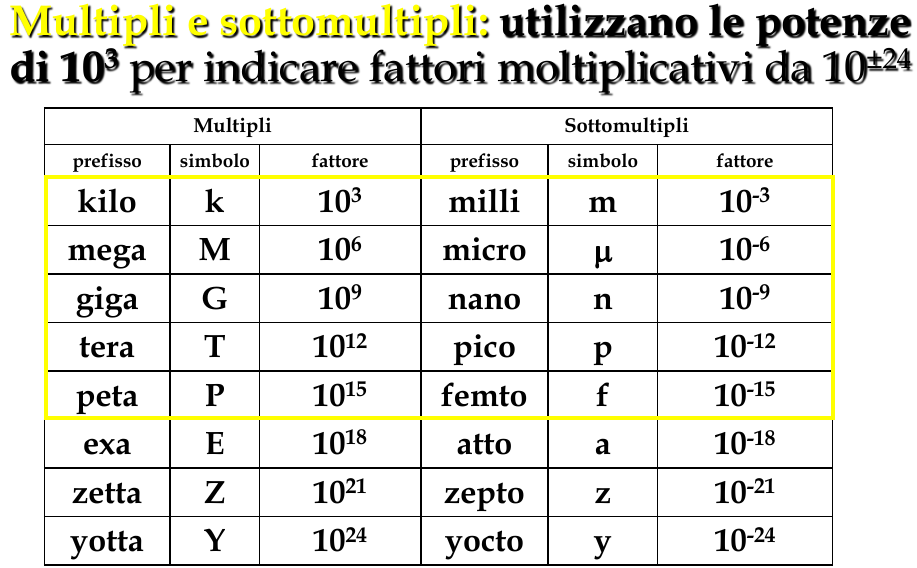
\includegraphics[
        width=12cm,
        height=6cm,
        keepaspectratio,
    ]{images/multiplisottomultipli.png}
    \caption{Multipli e Sottomultipli nel Sistema Internazionale.}
  \end{center}
\end{figure}
\section{Unità Logaritmiche} \label{sezione:unitaLog}
Le unità logaritmiche esprimono sotto forma di logaritmo il rapporto tra due grandezze \bf omogenee\rm. Notiamo che le grandezze in rapporto devono necessariamente essere omogenee, perché l'operatore logaritmo agisce solamente su numeri puri.
Una caratteristica che torna utile nelle unità logaritmiche è una delle proprietà dei logaritmi, cioè che le operazioni di moltiplicazione e divisione tra numeri si traducono in somme e differenze.

Le unità logaritmiche sono utilizzate molto el campo dell'elettronica e delle telecomunicazioni. I logaritmi più comunemente utilizzati sono quello in base 10 ($log_{10}$), quello in base $e$ ($log_{e} = ln$) e in informatica quello in base 2 ($log_{2}$).
\subsection{Il Bel}
Il \textbf{bel} esprime il rapporto di potenze in scala logaritmica utilizzando una base decimale: $$\Bigg(\frac{P_{2}}{P_{1}}\Bigg)_{(bel)} = log_{10}\Bigg(\frac{P_{2}}{P_{1}}\Bigg)$$
Il nome "bel" deriva dal suo inventore \textit{Alexander Graham-Bell} il quale, dovendo fare dei confronti tra potenze trasmesse per via aerea, si accorse che decadevano in maniera esponenziale.\\
È molto importante ricordarsi sempre che il bel rappresenta il logaritmo di un \textbf{rapporto tra due misure}, ed è quindi un modo per mettere in relazione due misure. Il difetto principale del bel è che 1 bel rappresenta un rapporto di un fattore 10:1 e dunque una scala in bel risulta "grossolana". Per risolvere\footnotemark \footnotetext[1]{Il significato di "risolvere" in questo caso è legato alla definizione che abbiamo dato nella sezione 1.3. Quindi "risolvere" in questo contesto và interpretato come "avere una \textbf{risoluzione} tale da poter apprezzare variazioni "più fini".} rapporti o variazioni "più fini" è conveniente utilizzare un suo \textbf{sottomultiplo}, il \textit{deciBel (dB)}.
\subsection{Il deciBel}
È un \textit{sottomultiplo} ($\frac{1}{10}$) del bel, esprime quindi anch'esso il rapporto di potenze (o anche ampiezze), mediante il logaritmo in base 10. $$\Bigg(\frac{P_{2}}{P_{1}}\Bigg)_{(dB)} = 10log_{10}\Bigg(\frac{P_{2}}{P_{1}}\Bigg)$$
Ricordando che il deciBel, come il bel, esprime rapporti di potenze, possiamo dire che $ 1\ dB \simeq 1.25 = 1 + 25\% $. Quindi si può dire che $P_{2}$ è "più grande" di $P_{1}$ del 25\%.\\
I rapporti di ampiezze, quando tensione e correnti sono misurate \textbf{su uno stesso carico}, si esprimono in deciBel secondo la relazione $$ 20log_{10}\Bigg(\frac{A_{2}}{A_{1}}\Bigg) $$
Questa formula discende direttamente dal decibel.$$Inserire\  dimostrazione?????$$
\subsection*{"dBx"}
Con dBx si indica il valore in decibel espresso rispetto ad un \textbf{riferimento x}. Scelto un livello di potenza $P_{x}$ come riferimento, un qualunque valore di potenza P può essere espresso in \textbf{decibel rispetto al riferimento} come
$$
  P_{(dBx)} = 10log_{10}\Bigg( \frac{P}{P_{x}} \Bigg)
$$
In particolare, esisterano dunque:
$$P_{(dBm)} = 10log_{10}\Bigg( \frac{P}{1mW} \Bigg)$$
$$P_{(dBW)} = 10log_{10}\Bigg( \frac{P}{1W} \Bigg)$$
$$P_{(dBk)} = 10log_{10}\Bigg( \frac{P}{1kW} \Bigg)$$
Che esprimono la variazione della potenza misurata rispetto ad un riferimento "standard" di 1 milliWatt, Watt oppure kiloWatt.\\ \\
Nota: i "dBx" sono normali decibel, quindi possono essere sommati/sottratti a decibel.\\ \\
{\Large {\textbf{Attenzione:}}} NON è in nessun modo sommare tra loro i dBx!! Un rapido esempio è che
$$1 W + 1 W = 2 W$$
$$+30 dBm + 30 dBm \neq + 60 dBm = \ kW$$
\subsection*{Calcoli Approssimati con i dB ????}
\subsection{Esempi di Calcoli e Conversioni con dB}
$$P = 10\ W \rightarrow P_{dBW} = 10 log_{10}\Bigg(\frac{P}{1W}\Bigg) = 10 log_{10}\Bigg(\frac{10 W}{1 W}\Bigg) = 10 log_{10}(10) = 10\ dBW$$
$$P = +90\ dBW = 10 log_{10}\Bigg(\frac{P}{1W}\Bigg) \rightarrow P = \Bigg( 10 \frac{PdbW}{10}\Bigg)\times 1 W = 10^9 W $$
\newpage
\chapter{Incertezza di Misura}
Abbiamo detto che la misura è un \textbf{numero} associato alla sua unità di \textbf{misura}. Adesso è il momento di aggiungere anche un qualcosa che esprime anche "quanto mi fido" della misura in questione, cioè l'\textbf{incertezza}. Possiamo quindi esprimere le misure, da ora in poi, come: $$ MIS_{x} = x_{numero}\ x_{unità\ di\ misura} \pm INC_{x}\ x_{unità\ di\ misura} $$
Addirittura a volte arriviamo ad esprimere anche l'incertezza dell'incertezza, che dice quanto fidarsi dell'incertezza. Esprime l'attendibilità della stima di incertezza in questione.
\section{Variabilità delle Misure} Misure ripetute dello stesso parametro fisico non forniscono lo stesso valore. È considerabile come una legge della natura, è impossibile che due misure consecutive diano esattamente lo stesso risultato per ogni cifra decimale. La caratteristica che ci permette di determinare l'incertezza della misura è la \textbf{deviazione standard} (o dispersione $\sigma$) della misura in questione, mentre il valore della misura sarà la \textbf{media} ($\mu$).
$$SLIDE\ GAUSSIANA$$
Le misure sono sempre affette da fluttuazioni o errori (almeno potenziali), mai perfettamente conoscibili, che si traducono in una naturale "indeterminazione" o INCERTEZZA sul risultato di misura.\\
Per questo conviene abbandonare l'approccio deterministico in favore di un \textbf{approccio statistico} grazie al quale è possibile stimare le fluttuazioni.\\
La variabilità del risultato di una misura è analizzata grazie ai metodi consolidati della statistica (varianza e deviazione standard). Il risultato dunque non è mai un unico numero "deterministico", ma un intervallo di valori possibili entro il quale il misurando può trovarsi con una data probabilità (e potrà anche trovarsi fuori dall'intervallo).
\paragraph*{Si definisce incertezza di misura} la semiampiezza di un particolare intervallo di valori (l'intervallo $\pm 1$ deviazione standard del valore centrale), centrato nella \textbf{media}.
\section{Teoria degli errori}
Anche se è ormai superata, la teoria degli errori di misura ci aiuta a comprendere la natura dell'incertezza, essa prevedeva che un misurando non potesse mai essere perfettamente conosciuto a causa degli inevitabili errori di misura (intrinseci in ogni metodo o strumento utilizzato per la misurazione). Si potrebbe dire che: $$Errore \equiv  Valore\ Misurato - Valore\ Vero$$
ma questa risulterebbe un'affermazione errata, dato che il valore \textbf{vero} non potrà mai essere conosciuto, esso è un mero concetto astratto, e quindi l'errore resta completamente indeterminato.\\
La teoria degli errori definiva alcuni tipi di errori che si verificano più spesso:
\begin{itemize}
  \item \textbf{Errori Sistematici:} si presentano nella stessa entità ogni volta che si ripete la misura (\textit{offset} o polarizzazione).\\
  Per esempio possiamo pensare ad un peso di massa \textit{m} che viene posto su una bilancia digitale, leggendo il valore riportato dalla bilancia si noterà un \textit{offset} costante di 100g in più rispetto al valore m.
  \item \textbf{Errori Accidentali:} si presentano in maniera diversa e "impredicibile" ogni volta che si ripete la misura (fluttuazione casuale a media nulla).\\
  Per esempio:
\end{itemize}
L'idea era sommare errori sistematici e accidentali, ma riflettendo un momento, anche se sappiamo che esse sono due grandezze omogenee, troviamo che sono concettualmente diverse per loro natura. È quindi logicamente scorretto sommarli in quanto i primi (sistematici, deterministici) sono completamente conscibili mentre i secondi (\textbf{aleatori}), sono solamente stimabili in senso statistico e talora riducibili ma \textbf{mai} eliminabili del tutto.
\paragraph*{Incertezza standard di misura} è ciò che secondo il CIPM è una corretta analisi statistica della variabilità di una misura. È un parametro, valutato seondo procedure \textbf{convenzionali} (standard), che esprime il nostro grado di non conoscenza del misurando.\\
Abbiamo due \textbf{categorie di stima} dell'incertezza:
\begin{itemize}
  \item \textbf{Stimata con Metodi Statistici} su un campione di misure.
  \item \textbf{Stimata in Altro Modo} ad esempio attraverso conoscenze a priori o proprietà dello strumento.
\end{itemize}
\section{Richiami di Probabilità e Statistica}
Per noi la probabilità è un numero $p\ \epsilon\ [0,1]$ dove 0 indica l'evento impossibile e 1 l'evento certo.\\
Chiamiamo invece \textit{variabile casuale} (VC) una variabile $X$ con valori $x\ \epsilon\ \Re $.\\
La probabilità è una funzione $P$ definita come:
$$P(a \le x \le b) \int^b_a p(x)dx$$
Cioè l'integrale tra due estremi $a$ e $b$ dell funzione $p(x)$ detta densità di probabilità (\textbf{PDF}). La PDF descrive il processo casuale considerato assegnando la probabilità per i possibili valori d'uscita. Per una VC continua la "probabilità puntuale" è nulla, mentre non può essere nulla la probabilità di cadere in un intervallo di valori. In altre parole, per una variabile aleatoria con PDF continua non è possibile che essa assuma un valore "deterministico", ma è solamente possibile ricavare la probabilità che il valore della VC stia in un intervallo di valori.\\
Per ogni PDF vale sempre $\int^{+\infty}_{-\infty}p(x)dx = 1$.\\

Per $X$ variabile casuale reale (che possiamo vedere come il possibile valore di una misura) esistono degli \textbf{stimatori} che ci consentono di conoscere, in senso statistico, alcuni parametri caratteristici del processo casuale. In particolare \textbf{media} e \textbf{varianza} permettono di stimare la tendenza centrale e la dispersione dei valore $x$ associabili a $X$.
\begin{itemize}
  \item \textbf{Media:}
  $$ \mu(x) = \mu_{x} = E[x] = \int^{+\infty}_{-\infty}xp(x)dx$$
    L'integrale di tutti i valori possibili di x pesati per il loro "peso probabilistico", cioè per la $p(x)$.
  \item \textbf{Varianza:}
  $$ \sigma^{2}(x) = \sigma^{2}_{x} = E[[x - \mu_{x}]^{2}] = \int^{+\infty}_{-\infty}[x - \mu_{x}]^{2}p(x)dx$$
  Scarto quadratico medio rispetto al "valore centrale", cioè la media.
  \item \textbf{Deviazione Standard:}
  $$ \sigma(x) = \sqrt{\sigma^{2}(x)} $$
  Indice di scarto, rispetto alla media, \textbf{lineare}.
\end{itemize}
\subsection{La PDF Gaussiana}
È la PDF "più comune" per la descrizione della media di fenomeni casuali quali le misure. Avendo infatti un significativo numero di misurazioni sappiamo, dalla statistica, grazie al teorema del limite centrale, che la media di una VC tende ad avere una PDF gaussiana in una "approssimazione dei grandi numeri". Assumendo quindi la PDF di una Gaussiana:\\
$$ p(x) = \frac{1}{\sqrt{2\pi}\sigma}e^{-\frac{[x-\mu]^2}{2\sigma^2}} $$
\begin{figure}[H]
  \begin{center}
    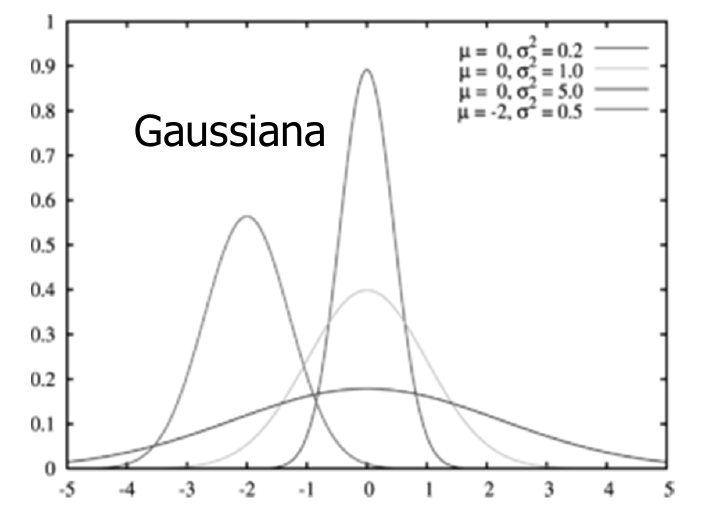
\includegraphics[
        width=10cm,
        height=5cm,
        keepaspectratio,
    ]{images/pdfgaussiana.png}
    \caption{La PDF gaussiana con vari esempi di valori di $\mu$.}
  \end{center}
\end{figure}
Integrando la PDF Gaussiana\footnotemark[1] \footnotetext[1]{In realtà la PDF Gaussiana non si può integrare analiticamente. Per fortuna però sono stati trovati dei modi per integrarla numericamente generando delle tabelle di valori di probabilità per diversi intervalli. Con espedienti di normalizzazione, riusciamo a calcolare le probabilità per tutte le $\infty^2$ Gaussiane esistenti.}tra due valori sull'asse reale si trova la probabilità che il risultato (misura) "cada" nell'intervallo compreso tra i due valori considerati.\\
Le \textbf{aree} sottese dalla PDF sono le probabilità di avere valori (misure) in un dato intervallo di valori sull'asse reale. Lontano dalla media $\mu$, rispetto alla larghezza $\sigma$, la PDF diviene molto bassa e dunque le aree sottese molto piccole, che implicano probabilità altrettanto "piccole", e rappresentano misure improbabili.
\begin{figure}[H]
  \begin{center}
    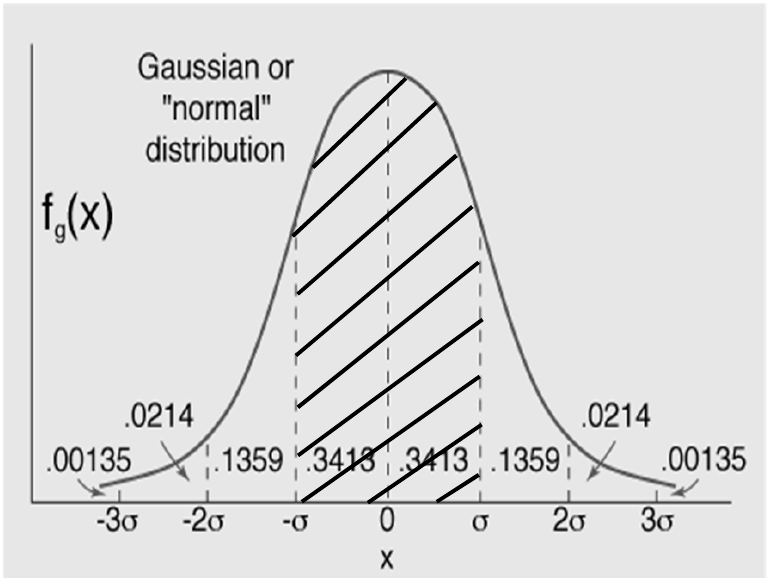
\includegraphics[
        width=10cm,
        height=5cm,
        keepaspectratio,
    ]{images/gaussianaIntervalli.png}
    \caption{La PDF gaussiana con vari livelli di confidenza.}
    \label{gaussiana:livelli}
  \end{center}
\end{figure}
\newpage
Il concetto di "vicinanza o lontananza dalla media" non si possono esprimere semplicemente attraverso i valori. Bisogna rapportare questi valori alla varianza $\sigma$: ad esempio, se sono lontano dalla media "di 10 milioni di kilometri" (che come valore è "molto grande" e quindi ci sembra di essere molto lontani), ma con una $\sigma$ di 100 milioni di kilometri, in realtà sono lontano dalla media solo di $\frac{\sigma}{10}$, quindi sono piuttosto vicino.


Livelli di confidenza è il nome che diamo a fattori moltiplicativi di $\sigma$ che indicano con quanta sicurezza cadremo in un intervallo di ampiezza $livello\ di\ confidenza \times \sigma$.
$$ 1\sigma \rightarrow 68.27\% \simeq 68.3\% \sim 68\% $$
$$ 2\sigma \rightarrow 95.45\% \simeq 95.5\% \sim 95\% $$
$$ 3\sigma \rightarrow 99.73\% \simeq 99.7\% \ \ \ \ \ \ \ \ \ $$
Per esempio, possiamo dire che la misura cadrà in un intervallo di ampiezza $1\sigma_{x}$ ripetto alla media $\mu_{x}$ con una \textbf{confidenza} del 68.3\%. In simboli:
$$ P[(\mu_x - \sigma_x)\le x \le (\mu_x + \sigma_x)] \simeq 68.3\% $$
Per un esempio grafico si può analizzare la Figura ~\ref{gaussiana:livelli}.
\subsection{Media Campionaria}
Sia $X$ una variabile casuale (il misurando), nota attraverso $n$ determinazioni (misure) $x_k\ (k=1,2,..n)$ ottenute in condizioni di \textbf{ripetibilità}, si \textbf{stima} del valor medio della "popolazione", $\mu(x)$, attraverso lo stimatore \textbf{media campionaria} (per lo specifico campione):
$$
  \bar{x} = \bar{x_k} \equiv \frac{1}{n} \sum^{n}_{k=1}x_k  
$$
Essendo questo uno stimatore, abbiamo anche che, \textit{nel senso della stima}, possiamo dire $ \mu_x = \bar{x}$.\\
A questo punto abbiamo determinato parte della misura così come la vogliamo noi. Abbiamo determinato il \textbf{valore di misura}. Per determinare la dispersione (incertezza) sul valore di misura dovremo valutare la dispersione, almeno potenziale, della variabile casuale $\bar{x}$ (valore di misura). Dunque cercheremo $\sigma(\bar{x})$, che scopriremo essere funzione di $\sigma(x)$ e del numero $n$ di misure ripetute.
\subsection{Varianza Campionaria}
Stimiamo la varianza della "popolazione", $\sigma^2$, attraverso lo stimatore \textbf{varianza campionaria} (per lo specifico campione):
$$
  s^2(x) = s^2(x_k) \equiv \frac{1}{n-1}\sum^{n}_{k=1}(x_k-\bar{x})^2
$$
Con pochi passaggi matematici si può arrivare anche al metodo alternativo per il calcolo della varianza campionaria:
$$
  s^2(x) = \frac{1}{n-1}\Bigg[\Bigg(\sum^{n}_{k=1}x^2_k\Bigg)-n\bar{x}^2\Bigg]
$$
\paragraph{Gradi di Libertà della Stima} è il nome che diamo all' $n-1$ nella formula della varianza, diremo che quella stima della varianza ha $v = n-1$ gradi di libertà.\\

\textit{Perché quindi dividiamo per il numero di gradi di libertà e non per n?}
\begin{itemize}
  \item Non ha alcun senso calcolare la varianza per un campione che contenga solo un dato ($n=1$) ed in tal caso, dividendo per $n-1 = 0$ si ottiene come $s^2(x)$ una forma indefinita del tipo $\frac{0}{0}$.
  \item Nella formula di $s^2(x)$ calcoliamo di fatto gli scarti quadratici dalla media campionaria, che è nota, e non dalla media della popolazione $\mu_x$ che è ignota: dunque degli $n$ scarti quadratici sommati solo $n-1$ sono tra loro indipendenti. Intuitivamente, conscendo la media di un campione di $n$ dati, ma conoscendo solamente $n-1$ di questi, si può facilmente ricavare l'$n-esimo$, quindi solo $n-1$ sono indipendenti.
  \item Si dimostra che il valore attteso della varianza campionaria con l'$n-1$ al denominatore, è la varianza della popolazione:
  $$
    E[s^2(x)] = \sigma^2(x)
  $$
  e si dice in questo caso che lo stimatore è \textit{corretto} (o non polarizzato).
\end{itemize}
\section{Incertezza Standard}
Possiamo ora definire l'\textbf{incertezza standard} (o scarto tipo):\\

Incertezza standard, con simbolo "$u$" (dall'inglese \textit{uncertainty}), è una \textbf{stima della deviazione standard} $\sigma$, radice quadrata della varianza $\sigma^2$, prevista per il valore di misura.\\ \\
A seconda del metodo impiegato per la stima di $u(\cdotp)$ classificheremo questa incertezza come di categoria A o B.

Ricordiamo che l'origine dell'incertezza dipende solamente dagli errori che abbiamo definito come \textit{accidentali}, non dalla parte sistematica, dato che quest'ultima (detta anche offset o polarizzazione) può essere sempre corretta.

\subsection{Incertezza di Categoria A}
Per determinare l'incertezza sul valore di misura valutiamo la deviazione standard della variabile casuale $\bar{x}$ (cioè del valore di misura).

$\bar{x}$ è, almeno potenzialmente, una variabile casuale in quanto il suo valore specifico dipende dal particolare campione di dati considerato. Se disponessimo di $m$ diversi insiemi di $n$ misure ripetute e per ciascuno calcolassimo la $\bar{x}$ corrispondente, otterremmo $m$ valori di $\bar{x}$ differenti tra loro, la cui varianza è:
$$
  \sigma^2(\bar{x}) = \sigma^2\Bigg(\frac{1}{n}\sum_kx_k\Bigg) = 
  \frac{1}{n^2}\sum_k\sigma^2(x_k) = \frac{1}{n^2}n\sigma^2(x) =
  \frac{\sigma^2(x)}{n}
$$
Quindi abbiamo che \textbf{la varianza del valor medio è la varianza dei dati diviso $n$}.
La \textbf{miglior stima} di $\sigma^2(\bar{x})$ si ottiene quindi come\footnotemark[1] \footnotetext[1]{$=^s$ va interpretato come "uguale nel senso della stima". I due termini infatti non sono uguali nel senso matematico del termine, ma \textbf{sotto un approccio statistico} possono considerarsi uguali.}:
$$
  \sigma^2(\bar{x}) = \frac{\sigma^2(x)}{n} =^s \frac{s^2(x)}{n}\ \ e\ \ \sigma(\bar{x}) = \frac{s(x)}{\sqrt{n}}
$$

Definiamo quindi l'\textbf{incertezza di categoria A} la dispersione del valor medio delle misure ripetute, calcolabile come:
$$
  u_A(x) = s(\bar{x}) = \frac{s(x)}{\sqrt{n}} = \sqrt{\frac{1}{n(n-1)}\sum^n_{k=1}(x_k-\bar{x})^2}
$$

Nel caso di incertezza \textbf{solo} di categoria A, il risultato di misura è allora $x = \bar{x} \pm \frac{s(x)}{\sqrt{n}}$, con una qualità che migliora (quindi l'incertezza diminuisce) al crescere di $n$.
\subsection{Incertezza Relativa}
Parleremo di \textbf{incertezza relativa} quando normalizziamo il valore di incertezza dipo al valore di misura:
$$
  u_r(x) = \frac{u(x)}{\bar{x}}
$$
Dimensionalmente è un \textbf{numero puro}.

L'incertezza relativa indica, indipendentemente dal valore e tipo del misurando, il grado di conoscenza che abbiamo raggiunto sul \textbf{valore di misura}. Essendo quindi un parametro relativo solamente al \textbf{valore}, possiamo confrontare direttamente tra loro incertezze relative di grandezze diverse (non omogenee), perché non trattiamo di unità di misura. Un esempio può essere: possiamo confrontare l'incertezza relativa su una misura di un intervallo di tempo (una \textit{parte per milione} - $10^{-6}$) con l'incertezza relativa della misura dell'altezza di un edificio ($10^{-3}$) dicendo che la prima misura è sicuramente \textbf{migliore} della seconda, in termini di incertezza.

Ora che conosciamo l'incertezza relativa, possiamo \textit{"relativizzare"} qualunque tipo di incertezza, anche quella che vediamo al prossimo paragrafo, l'\textbf{incertezza estesa}.
\subsection{Incertezza Estesa}
Con l'incertezza estesa definiamo un intervallo di valori centrato nel valore di misura $y = \bar{y}$ all'interno del quale si ritiene che il misurando debba cadere con un certo \textbf{livello di confidenzza}.
$$
  U(y) = k u(y)
$$
Con $k$ \textit{fattore di copertura}. I valori che tipicamente assume $k$ sono 1,2 e 3, che corrispondono rispettivamente a livelli di confidenza del 68, 95, 99.7\%.

Questo si può desumere intuitivamente, l'incertezza come l'abbiamo definita va ad indicarci un intervallo di valori attorno al valore di misura nel quale è contenuto il "vero" valore della misura. Con l'incertezza estesa andiamo appunto ad \textit{estendere} questo intervallo di un fattore "a piacere", aumentando la probabilità che il valore "vero" vi sia contenuto.
\subsection{Cifre signifiative per l'incertezza}
Abbiamo già menzionato l'esistenza dell'"incertezza dell'incertezza", definendola come un parametro indicattivo del nostro livello di fiducia del calcolo dell'incertezza. Già questo fatto suggerisce che l'incertezza che calcoliamo non può essere espressa molto precisamente.

Infatti, l'incertezza si esprime con una o \textbf{al più due} cifre significative: data l'esistenza di un'incertezza dell'incertezza non ha senso impiegare più di due cifre significative per $u(x)$. Quando si deve troncare il valore di un'incertezza, è necessario \textbf{arrotondare per eccesso}, a meno che l'arrotondamento per difetto non comporti un errore inferiore al 5\%. Questo perché non vogliamo \textbf{sottostimare} l'incertezza, dato che potrebbe comportare errori gravi, vorrebbe dire che il valore "vero" della misura potrebbe cadere al di fuori dell'intervallo da noi definito "molto più frequentemente" di quanto ci aspettiamo. Per questo è sempre meglio \textbf{sovrastimarla} arrotondando per eccesso.

Un esempio di arrotondamento per difetto che comporta meno del 5\% di errore può essere:
$$
  u(m) = 89.1\ kg\ = 89\ kg
$$
perchè in questo caso lo 0.1 su 89 kilogrammi è sicuramente meno del 5\%.
\subsection{Esercizio: Calcolo Incertezza di Cat. A}
Si dispone di n = 10 misure ripetute $V_k$ di una tensione incognita $V$.\\
Calcolare $V$ $u_A(V)$.
\begin{table}[H]
  \caption{Serie di misurazoni da considerare.}
  \label{tab:esIncertezza}

  \begin{center}
    \begin{tabular}{|l|c|r|r|r|r|r|r|r|r|r|}
    \hline
       k[1]       & 1& 2& 3& 4& 5& 6& 7& 8& 9& 10 \\
    \hline
       $V_k$[$V$] & 7& 9& 8& 6& 7& 5& 7& 8& 6& 7 \\
    \hline
    \end{tabular}
  \end{center}
\end{table}
Calcoliamo la media campionaria per conoscere il valore medio che è il valore della nostra misura:
$$
  V = \bar{V} = \frac{1}{n}\sum^n_{k=1}V_k = \frac{1}{10}70\ V = 7 V
$$
Posso quindi calcolare l'incertezza standard di categoria A per la misura con ognuna delle seguenti formule:
\begin{align}
  u_A(V)& = \frac{s(V)}{\sqrt{n}} \label{incA:1}\\
  u_A(V)& = \sqrt{\frac{1}{n(n-1)}\sum^n_{k=1}(V_k-\bar{V})^2} \label{incA:2}\\
  u_A(V)& = \sqrt{\frac{1}{n(n-1)}\Bigg(\sum^n_{k=1}(V_k^2)\Bigg)-n\bar{V}^2} \label{incA:3}
\end{align}

Per la seconda espressione (Formula \ref{incA:2}) di $u_a(V)$ ci conviene prima calcolare tutti gli scarti $(V_k-\bar{V})$, notando che alcuni degli scarti che otteniamo risultano 0 e quindi non contribuiscono all'incertezza\footnotemark[1].\footnotetext[1]{Se invece l'intera incertezza standard di categoria A dovesse risultare 0, vuol dire che abbiamo commesso uno o più errori. Ad esempio, se le misurazioni effettuate variavano al millivolt, mentre sono state annotate al volt, la causa dell'errore è l'operatore che non ha annotato correttamente le misurazioni.}
\begin{table}[H]
  \caption{Scarti calcolati rispetto alla media campionaria $\bar{V}$.}
  \label{tab:esIncertezza:scarti}

  \begin{center}
    \begin{tabular}{|l|c|r|r|r|r|r|r|r|r|r|}
    \hline
       ($V_k-\bar{V}$) [$V$]   & 0& 2& 1& -1& 0& -2& 0& 1& -1& 0 \\
    \hline
    \end{tabular}
  \end{center}
\end{table}
Ricaviamo quindi:
$$
  u_A(V) = \sqrt{\frac{1}{10\times 9}(0+4+1+1+0+4+0+1+1+0)V^2} = \sqrt{\frac{12}{90}V^2} \simeq 0.37\ V
$$
\\
Per la terza espressione (Formula \ref{incA:3}), calcoliamo prima la sommatoria
$$
  \sum^N_{k=1}V^2_k = 502\ V^2\ e\ \bar{V} = 7\ V
$$
ricavando quindi:
$$
  u_A(V) = \sqrt{\frac{1}{10\times 9}[509\ V^2 - 10 \times 49\ V^2]} = \sqrt{\frac{12}{90}\ V^2} \simeq 0.37\ V
$$
\\
Per la prima espressione (Formula \ref{incA:1}) dobbiamo prima conoscere o calcolare la radice della varianza campionaria (cioè la deviazione standard campionaria) $s(V) = 1.1547$ per poi dividerla per $\sqrt{n}$:
$$
  u_A(V) = \frac{1.1547\ V}{\sqrt{10}} = 0.365148... \simeq 0.37\ V
$$

In questo ultimo caso abbiamo un esempio di arrotondamento dell'incertezza alla seconda cifra decimale, per eccesso. Ma se, ad esempio, il risultato fosse stato 0.36\textbf{4}321? Questo 4 come terza cifra decimale ci avrebbe permesso di arrotondare il risultato per difetto? Ovviamente no, perchè avrebbe comportato un errore molto maggiore rispetto al 5\%.
\subsection{Cifre significative per il risultato di una misura}
Esistono due maniere per esprimere una misura, in forma estesa e in forma compatta, con i numeri dell'esercizio precedente avremmo:
\begin{center}
  V = 7.00 V $\pm$ 0.37 V~~ oppure~~ V = 7.00(37) V    
\end{center}
O anche, in modo più approssimato: V = 7.0 V $\pm$ 0.4 V.
\subsection{Incertezza di Categoria B}
Si basa sulla definizione "a priori" di un opportuno intervallo di valori entro il quale si suppone debbano cadere i valore del misurando (con una data probabilità). L'intervallo non viene naturalmente definito "a caso", ma si presuppone di conscerlo da studi antecedenti alla misura.

L'intervallo fissato è tipicamente centrato attorno al \textbf{valor medio}
$$\bar{x} = a_0 = \frac{(a_0+a)+(a_0-a)}{2}$$ ed ha una piena larghezza $$\Delta x = (a_0+a)-(a_0-a) = 2a$$
E chiaramente alla larghezza $\Delta x$ sarà legata l'\textbf{incertezza di misura}.\\
Questo intervallo viene modellizzato con una \textbf{PDF} di cui possiamo calcolare media $\mu$ e varianza $\sigma^2$. Ad esempio possiamo modellizzare con una ben nota Gaussiana Standard con $2\sigma = $ l'ampiezza dell'intervallo. Ma in altri casi è possibile che i ragionamenti "a priori" ci diano motivo di pensare che la PDF migliore sia \textit{triangolare}, oppure \textit{uniforme}.\\

Dunque possiamo definire il procedimento per ottenere una stima dell'incertezza standard di categoria B:
\begin{enumerate}
  \item Definito un \textbf{intervallo} di categoria B
  \item si associa una densità di probabilità (\textbf{PDF})
  \item di questa si calcolano media $\mu$, varianza e \textbf{deviazione standard} $\sigma$.
\end{enumerate}
\begin{figure}[H]
  \begin{center}
    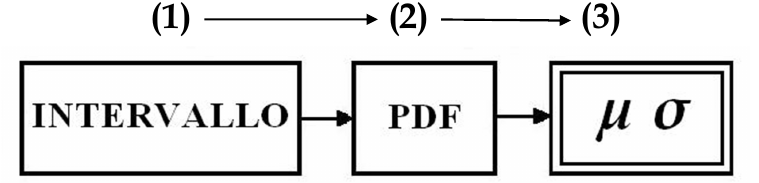
\includegraphics[
        width=10cm,
        height=5cm,
        keepaspectratio,
    ]{images/passiIncertezzaB.png}
    \caption{Passi per l'incertezza standard di categoria B.}
    \label{incertezzaB:passi}
  \end{center}
\end{figure}
Ma a questo punto una domanda sorge spontanea:
\begin{center}
  \textit{Come segliamo l'intervallo e la PDF?}
\end{center}
Tanto la larghezza dell'intervallo quanto la PDF ad esso associata si scelgono sulla base di:
\begin{itemize}
  \item precedenti conosenze o dati di misura
  \item esperienza sul comportamento del misurando
  \item specifiche dei costruttori di materiali e strumenti coinvolti nella misura
  \item dati di calibrazioni
  \item informazioni da articoli scientifici/tecnici
  \item incertezza sui parametri di riferimento (presa dai manuali o da altre fonti)
\end{itemize}
\subsection{Le PDF più comuni}
\subsubsection{Gaussiana (Normale)}
Basta ricordare che
\begin{center}
\begin{itemize}
  \item $1\sigma$ \textit{level}: $P[\mu-\sigma \le x \le \mu+\sigma] \simeq 68.3\%$
  \item $2\sigma$ \textit{level}: $P[\mu-2\sigma \le x \le \mu+2\sigma] \simeq 95.5\%$
    \item $3\sigma$ \textit{level}: $P[\mu-3\sigma \le x \le \mu+3\sigma] \simeq 99.7\%$
\end{itemize}  
\end{center}
\subsubsection{Uniforme (Rettangolare)}
La PDF rettangolare è definita come:
\begin{equation}
   \begin{cases}
   0~~~~~~~~~~~~~~~x < a_0 -a\\
   \frac{1}{2a}~~~~~~~~~~~~~a_0 -a \le x \le a_0 + a\\
   0~~~~~~~~~~~~~~~x > a_0 +a
   \end{cases}
\end{equation}
La particolarità della PDF uniforme è che si può \textbf{sempre} esprimere la sua deviazione standard come:
$$
  \sigma_{UNI}(x) = \frac{\Delta x}{\sqrt{12}}
$$
\subsubsection{Triangolare}
Elenchiamo alcune delle proprietà della PDF Triangolare
$$
  \mu(x) = a_0
$$
Con $a_0$ valore medio.
$$
  \sigma^2(x) = \frac{a^2}{6} = \frac{(\Delta x)^2}{24}
$$
$$
  \sigma(x) = \frac{\Delta x}{\sqrt{24}}
$$
A pari larghezza $\Delta x$, si ha naturalmente che:
$$
  u_{B,triangolare}(x) = \frac{\Delta x}{\sqrt{24}} < u_{B,uniforme}(x) = \frac{\Delta x}{\sqrt{12}}
$$
Infatti la PDF$_{Tri}$ è "meno dispersa" della PDF$_{Uni}$.
\newpage
\section{Incertezza Composta $u_C$}
L'incertezza composta deriva appunto dalla composizione di incertezza di categoria A e di categoria B.
\subsection{Incertezza Composta per Misure Dirette e indirette}
\subsubsection{Misure Dirette}
Nel caso di misure dirette (\textit{e.g.} misure di V con un voltmetro) possiamo calcolare l'incertezza composta come:
$$
  u^2_C = u^2_A + u^2_B
$$
\subsubsection{Misure Indirette}
Nel caso di misure \textbf{indirette}, invece, il discorso è molto più complesso.

Un esempio di misura indiretta piò essere la misura di una potenza elettrica \textbf{senza wattmetro}, cioè ottenuta da R ed I tramite la formula $P = RI^2$. In questo caso la \textbf{misura è funzione di più misure}: $y = f(x_1,x_2,\ldots ,x_N)$
È possibile calcolare $u_B(x)$ partendo dalla conoscenza di un \textbf{ intervallo di confidenza} con probabilità $P$, usando una PDF notmale con confidenza $P$, centrata sul valore centrale dell'intervallo.

Stimeremo l'incertezza in questo caso come:
$$
  u_B(x) = \sigma(x) = \sigma_x
$$\\

In altri casi si può calcolare $u_B(x)$ partendo dalla conoscenza di una \textbf{incertezza estesa} $U_B = k u_B$, conoscendo il fattore di copertura $k$. Dalla definizione di incertezza estesa possiamo quindi ricavare $u_B(x)$ come:
$$
  u_B(x) = \frac{U_B(x)}{k}
$$
Definiamo le componenti delle misure indirette:
\begin{itemize}
  \item \textbf{Misurando}: $Y = f(X_1,X_2,\ldots,X_N)$ ricavato \textbf{indirettamente} dalla conoscenza di N altre grandezze (dette parametri di ingresso)
  \item \textbf{Relazione Funzionale} (o equazione della misura): la funzione $f(X_i)$
  \item Ricordiamo inoltre che $Y$ e $X_i$ sono le variabili, mentre $y$ e $x_i$ i valori delle variabili
\end{itemize}
Naturalmente dalla conoscenza dei valori degli ingressi è possibile ricavare il \textbf{valore dell'uscita}: $y = f(x_i)$.

Saranno invece le \textbf{incertezze degli ingressi}, opportunamente combinate, a fornire l'\textbf{incertezza dell'uscita}:
$$
  u_C(y) = \Phi[u(x_i);f(\cdotp)]
$$
Dati i valori della relazione funzionale, è possibile sviluppare in \textbf{serie di Taylor} al primo ordine la relazone funzionale $f$ in un intorno del valore di misura (o \textbf{punto di lavoro}):
$$
  (y-\bar{y}) \simeq \Bigg(\frac{\delta f}{\delta x_1}\Bigg)_{\bar{y}} (x_1 + \bar{x_1})+\ldots+\Bigg(\frac{\delta f}{\delta x_N}\Bigg)_{\bar{y}} (x_N + \bar{x_N}) 
$$
Definiamo quindi \textbf{coefficienti di sensibilità} le derivate prime parziali della relazione funzionale rispetto alla variabile $x_i$:
$$
  c_i \equiv \Bigg(\frac{\delta f}{\delta x_1}\Bigg)_{\bar{y}}
$$
$c_i$ indica come varia il bisurando $Y$ in corrispondenza di una variazione del parametro $X_i$ di dipendenza.
\subparagraph*{Covarianza:} definiamo covarianza (con $i \ne j$):
$$
  E \Bigg[(x_i - \bar{x_i})(x_j - \bar{x_j})\Bigg] \equiv \sigma^2(x_i,x_j) = u (x_i,x_j)
$$

Possiamo quindi scrivere l'espressione dell'incertezza composta al quadrato come:
$$
  u_C^2 = \sum^N_{i = 1}\Bigg(\frac{\delta f}{\delta x_i}\Bigg)^2 u^2(x_i)+2\sum^{N-1}_{i = 1}\sum^{N}_{j = i +1}\Bigg(\frac{\delta f}{\delta x_i}\Bigg)\Bigg(\frac{\delta f}{\delta x_j}\Bigg)u(x_i,x_j)
$$ dove:
$$
  \Bigg(\frac{\delta f}{\delta x_i}\Bigg)^2
$$
è la somma pesata, con pesi $c_i^2$, delle incertezze (varianze) degli ingressi $x_i$ più la somma dei termini di \textit{covarianza}, sempre pesati con le derivate prime della relazione funzionale.

Possiamo affermare a questo punto che il \textbf{valore della misura} della grandezza $Y$ è:
$$
  y = \bar{y} = f(\bar{x_1},\bar{x_2},\ldots,\bar{x_N})
$$ ed ha una \textbf{incertezza composta} che vale:
$$
  u_c(y) = \sqrt{  u_C^2 = \sum^N_{i = 1}c_i^2 u^2(x_i)+2\sum^{N-1}_{i = 1}\sum^{N}_{j = i +1}c_i c_j u(x_i,x_j)}
$$
Sappiamo anche che in generale ciascuna incertezza $u(x_i)$ è:
$$
  u_c(x_i) = \sqrt{u_A^2(x_i)+u_B^2(x_i)} = \sqrt{s^2(\bar{x_i})+u_B^2(x_i)} = \sqrt{\frac{s^2(x_i)}{n}+u_B^2(x_i)}
$$
Per arrivare a semplicifare la formula dell'uncertezza combinata, andiamo a definire i \textbf{coefficienti di correlazione}:
$$
  i_{ij}(x_i,x_j) \equiv \frac{u(x_i,x_j)}{u(x_i)\cdot u(x_j)}~\epsilon [-11;+1]~
$$ definito come il rapporto tra la covarianza di due variabili e il prodotto delle loro varianze. È importante notare che se $X_i$ e $X_j$ sono variabili aleatorie tali per cui il comportamento di una non influisce sulla variazione dell'altra (cioè sono \textbf{statisticamente indipendenti}), allora il loro coefficiente di correlazione sarà pari a 0.
$$
    r_{ij} = 0~~~~\text{se $X_i$ e $X_j$ sono statisticamente indipendenti}
$$
Nel caso di \textbf{variabili d'ingresso statisticamente indipendenti} tutti i termini di covarianza e i coefficienti i correlazione sono nulli ($r_{ij} = 0$ tra le variabili $x_i$ e $x_j$ con $i \neq j$) e pertanto:
$$
  u_c(y) = \sqrt{\sum^{N}_{i_1}\Bigg(\frac{\delta f}{\delta x_i}\Bigg)^2 u^2(x_i)}
$$ e quindi:
$$
  u^2_c(y) = \sum^{N}_{i = 1}c_i^2 u^2 (x_i)
$$ risulta essere una \textit{somma di varianze}.

Nella maggior parte dei casi analizzati riusciremo a dedurre che le variabili d'ingresso sono statisticamente indipendenti, quindi potremo applicare queste ultime due formule.
\subsubsection{Casi Particolari di Relazioni Funzionali}
Nei due seguenti casi abbiamo che le variabili d'ingresso $X_i$ sono statisticamente indipendenti:
\begin{itemize}
  \item Misurando somma o differenza delle $x_i$:
  $$
    \bar{y} = n_1\bar{x_1}\pm\ldots n_i\bar{x_i}\pm\ldots n_N\bar{x_N}
  $$
  $$
    u^2_c(y) = \sum^N_{i = 1}n_i^2 u^2(x_i)
  $$
  Se inoltre $n_i = 1$ per ogni $i$, cioè la relazione funzionale è una somma algebrica semplice:
  $$
    u_c(y) = \sqrt{\sum^N_{i = 1}u^2(x_i)}
  $$
  \item Misurando prodotto o rapporto delle $x_i$:
  $$
    u{r,c}(y) = \sqrt{\sum^{N}_{i = 1}n_i^2 u_r^2(x_i)}
  $$
    Se inoltre $n_i = 1$ per ogni $i$, cioè la relazione funzionale è espressa da prodotti e rapporti semplici:
    $$
      u_{r,c}^2(y) = \sum^{N}_{i = 1}u_r^2(x_i)
    $$
\end{itemize}
\subsection{Esercizio di Esempio: Legge dei Gas Perfetti}
La relazione funzionale è:
\begin{equation}
  \label{gas perfetti}
  p = n \frac{RT}{V} = f (n,R,T,V)
\end{equation}

dove:
\begin{itemize}
  \item $R = 8.31~\Bigg[\frac{Pa\cdot m^3}{mol\cdot k}\Bigg]$~~~ con $u(R) \simeq 0$ (trascurabile per il nostro problema)
  \item $n = 2~mol$~~~~ con $u_r(n) = 10^{-6}$
  \item $T = 300~K$~~~ con $u(T) = 0.1 K$
  \item $V = 1~m^3$~~~~~ da $V = L^3$ e $L = 1~m\pm 1~mm$
\end{itemize}
Possiamo immediatamente calcolare il \textbf{valore} della misura:
$$
  p = \frac{2~[mol]\cdot 8.31~\Bigg[\frac{Pa\cdot m^3}{mol\cdot k}\Bigg]\cdot 300~[K]}{1~[m^3]} = 4986~Pa \simeq 5~kPa
$$
Per calcolare l'incertezza innanzitutto ci accorgiamo che è necessario calcolare una incertezza composta, con relazione funzionale espressa nella Formula \ref{gas perfetti}. Per calcolare questa quindi necessitiamo di sapre le incertezze di tutte le variabili coinvolte nella relazione funzionale.

L'incertezza di R è trascurabile per ipotesi, quella di n è nota così come quella di T, ma non conosciamo l'incertezza di V. Procediamo quindi a calcolarla: anche questa in un certo senso è il calcolo di un incertezza composta, con la relazione funzionale $ V = L^3 $, quindi scriviamo:
$$
  u(V) = \sqrt{\Bigg(\frac{\delta V}{\delta L}\Bigg)^2 u^2(L)} = \sqrt{[3~m^2]^2\cdot[10^{-3}~m]^2} = \sqrt{9\times 10^{-6}~m^6} = 3\times 10^{-3}~ m^3
$$
Ora, conscendo tutte le variabili/grandezze d'ingresso per valore ed incertezza, possiamo calcolare l'incertezza composta della grandezza misurata indirettamente:
\begin{align*}
&u(p) = \sqrt{\Bigg(\frac{\delta p}{\delta n}\Bigg)^2 u^2(n)+\Bigg(\frac{\delta p}{\delta T}\Bigg)^2 u^2(T)+\Bigg(\frac{\delta p}{\delta V}\Bigg)^2 u^2(V)} =\\
&= \sqrt{\Bigg(\frac{RT}{V}\Bigg)^2 u^2(n)+\Bigg(\frac{nR}{V}\Bigg)^2 u^2(T)+\Bigg(\frac{nRT}{-V^2}\Bigg)^2 u^2(V)} =\\
&= \sqrt{\Bigg(\frac{nRT}{V}\Bigg)^2 \frac{u^2(n)}{n^2}+\Bigg(\frac{nRT}{V}\Bigg)^2 \frac{u^2(T)}{T^2}+\Bigg(\frac{nRT}{-V}\Bigg)^2 \frac{u^2(V)}{V^2}}\\
\end{align*}
Dall'ultima espressione possiamo concludere che:
\begin{equation}
\label{formula incertezza composta}
  u_r(p) = \sqrt{u_r^2(n)+u_r^2(T)+u_r^2(V)}
\end{equation}
Questa sarà quindi la formula da usare non solo in questo caso, ma anche in tutti gli altri casi simili a questo!

Per concludere:
\begin{itemize}
  \item $u_r^2(n) = 10^{-12}$
  \item $u_r^2(T) = \frac{(0.1~K)^2}{(300~K)^2} \simeq 1.1\times 10^{-7}$
  \item $u_r^2(V) = \frac{3\times 10^{-3}~ m^3)^2}{(1~m^3)^2} \simeq 9\times 10^{-6}$
\end{itemize}
e quindi:
\begin{equation}
  \label{calcolo p}
  u_r(p) = \sqrt{10^{-6}(10^{-6}+0.11+9)} \simeq 3\times 10^{-3}
\end{equation}
e inoltre:
$$
  u(p) = u_r(p)\times p = 14.9~ Pa \simeq 15~Pa
$$
Possiamo in conclusione esprimere la misura completa della sua incertezza inelle due notazioni:
$$
  p = 4986~ Pa\pm 15~ Pa = 4986(15)~ Pa
$$
\subparagraph{Nota} come possiamo notare dalla Formula \ref{calcolo p} e dalla \ref{forumla incertezza composta}, l'incertezza relativa di $p$ risulta essere pressochè identica all'incertezza relativa di $V$. Questo perchè $u_r(V)^2$ è il termine predominante sotto la radice. Avremo \textbf{sempre}, quindi, che se un termine particolare è superiore agli altri di almeno un fattore 5, esso risulterà come termine dominante e l'incertezza relativa risultante protrà essere approssimata ad esso.
\chapter{Rappresentazione Grafica dei Risultati Sperimentali - Interpolazione e Curve di Regressione}
\section{Rappresentazione Grafica dei Risultati Sperimentali}
La rappresentazione grafica di effettua per ottenere una "visione d'insieme" di una grandezza, inf unzione del tempo (o di un altro parametro). Si utilizzano tipicamente assi coortinati che devono riportare la descrizione della grandezza rappresentata e all'occorrenza \textbf{anche la sua unità di misura}.

Si distinguono infatti due tipi di grafici:
\begin{itemize}
  \item Grafici \textbf{quantitativi}: grafici in cui sugli assi compaiono dei valori numerici, dei quali bisogna sempre indicare l'unità di misura corrispondente.
  \item Grafici \textbf{qualitativi}: i grafici che non sono quantitativi si dicono qualitativi, e sono spesso usati per indicare degli andamenti o delle tendenze.
\end{itemize}
\paragraph{Grafico in un piano cartesiano}~\\
Come già si dovrebbe sapere, il grafico in un piano cartesiano è composto da due assi, uno per le \textit{ascisse} e uno per le \textit{ordinate}. Sull'asse delle \textit{ascisse} (asse X) ci sarà la variabile \textbf{indipendente}, anche detta "comando d'ingresso"- Sull'asse delle \textit{ordinate} (asse Y) ci sarà invece la variabile \textbf{dipendente}, anche detta "grandezza d'uscita".

Va notato che tipicamente avremo $u(x_i) << u(y_i)$, ossia la variabile di comando è nota con buona precisione (diremo che ha incertezza trascurabile), mentre la variabile di uscita presenta una maggiore incertezza, che andrà rappresentata su grafico tramite delle \textit{\textbf{barre d'errore}}. Possiamo vedere un esempio di queste barre d'errore bella Figura: \ref{rappresentazione:barrerrore}, nella quale le barre indicano un intervallo di confidenza, che va specificato: ad esempio scriveremo in aggiunta al grafico che esse rappresentano un intervallo di confidenza del $\pm 1 \sigma$ (68\%).
\begin{figure}[H]
  \begin{center}
    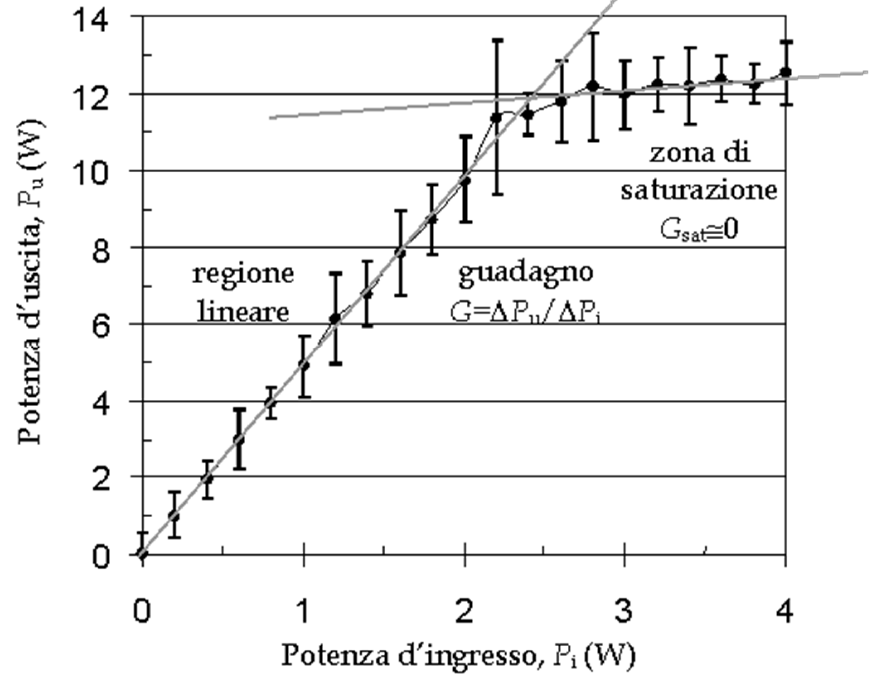
\includegraphics[
        width=16cm,
        height=7cm,
        keepaspectratio,
    ]{images/esempioBarreErrore.png}
    \caption{Caratteristica ingresso-uscita di un amplificatore elettronico.}
    \label{rappresentazione:barrerrore}
  \end{center}
\end{figure}
\paragraph{Grafico in un Diagramma Polare}~\\
In alternativa ai diagrammi cartesiani, per alcuni casi si usano i diagrammi polari, in cui abbiamo sempre due coordinate, ma sono una radiale e l'altra angolare.
\begin{itemize}
  \item Coordinata radiale: $\rho = \sqrt{(x^2+y^2)} $
  \item Coordinata angolare: $\theta = \arctan(\frac{y}{x})~~per~~x\ge 0$
\end{itemize}
Quindi avremo:
\begin{itemize}
  \item $x = \rho \cos(\theta) $
  \item $y = \rho \sin(\theta) $
\end{itemize}
Nella Figura \ref{rappresentazione:diagrammaPolare} possiamo vedere un esempio in cui viene utile utilizzare un diagramma polare per la rappresentazione dei dati. Il diagramma mostra la direttività di un altoparlante e si può facilmente vedere come, immaginando che l'altoparlante si trovi all'origine degli assi diretto "verso l'alto" (verso la direzione delle $y$ crescenti) se ci si posiziona \textbf{dietro} di esso (cioè nella parte negativa dell'asse $y$) il suono viene propagato molto poco e per direzioni ridotte, mentre viene ben amplificato e propagato nella parte positiva dell'asse $y$.
\begin{figure}[H]
  \begin{center}
    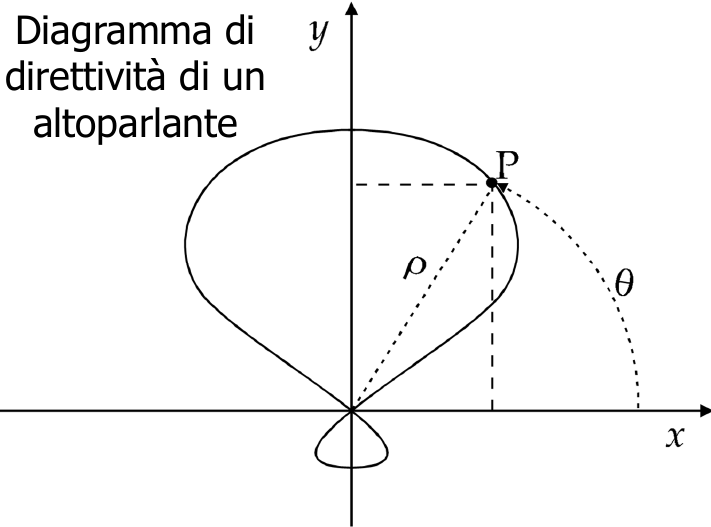
\includegraphics[
        width=16cm,
        height=7cm,
        keepaspectratio,
    ]{images/diagrammaPolare.png}
    \caption{Un esempio di diagramma polare.}
    \label{rappresentazione:diagrammaPolare}
  \end{center}
\end{figure}
\paragraph{Grafico in scala semilogaritmica}~\\
Come già studiato nella Sezione \ref{sezione:unitaLog}, le unità logaritmiche sono utili per visualizzare grandezze che variano di diversi ordini di grandezza, con dettaglio relativo costante, cioè punti equispaziati in scala logaritmica stanno in uno \textbf{stesso rapporto} in scala lineare.

I diagrammi \textit{semi}logaritmici sono tali perché hanno uno degli assi in scala logaritmica, mentre l'altro in scala lineare. In Figura \ref{diagrammi:semilogy} possiamo vedere un diagramma "\textit{semilog-}$y$" per la curva I-V di un diodo a semiconduttore in polarizzazione diretta: $I = I_0 e^(\frac{V}{V_T})$
\begin{figure}[H]
  \begin{center}
    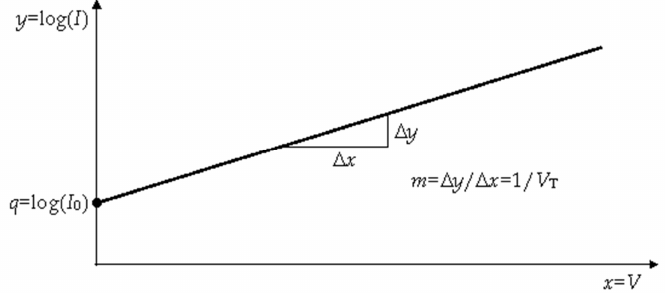
\includegraphics[
        width=8cm,
        height=7cm,
        keepaspectratio,
    ]{images/semilog.png}
    \caption{Un esempio di diagramma semilogaritmico.}
    \label{diagrammi:semilogy}
  \end{center}
\end{figure}
Un ulteriore esempio di diagramma semilogaritmico è un diagramma di Bode della fase\footnotemark[1]\footnotetext[1]{I diagrammi di Bode della fase e del Modulo verranno trattati approfonditamente nel corso di Automatica.}, mostrato in figura \ref{diagrammi:BodeFase}, che rappresenta lo sfasamento in gradi (o radianti) sull'asse verticale in funzione della frequenza riportata in scala logaritmica sull'asse orizzontale (dato che spesso per le componenti analizzate in questi diagrammi si ha un'ampia dinamica di frequenza).
\begin{figure}[H]
  \begin{center}
    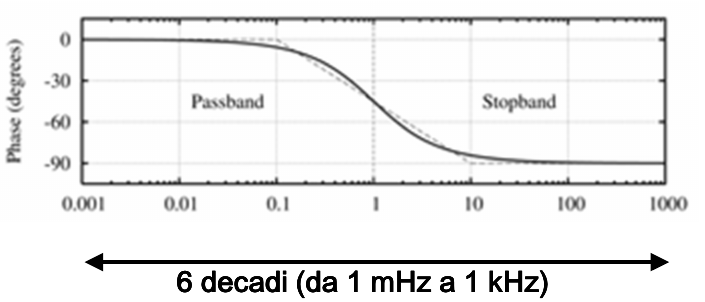
\includegraphics[
        width=8cm,
        height=7cm,
        keepaspectratio,
    ]{images/bodeFase.png}
    \caption{Un esempio di diagramma di Bode della Fase.}
    \label{diagrammi:BodeFase}
  \end{center}
\end{figure}
\paragraph{Grafico in scala semilogaritmica}~\\
Quando si ha necessità di rappresentare ampie dinamiche di funzione per entrambe le variabili di controllo e controllata, si può ricorrere all'uso di diagrammi "interamente" logaritmici (\textit{log-log}). Come per esempio viene fatto nel diagramma di Bode del Modulo\footnotemark[1] per rappresentare l'ampiezza o guadagno in dB in funzione delle afrequenza riportata in scala logaritmica (vedi Figura \ref{diagrammi:BodeModulo}).
\begin{figure}[H]
  \begin{center}
    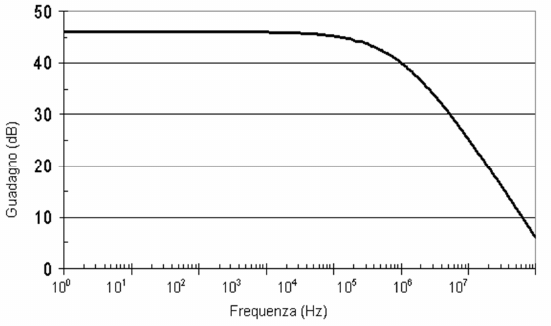
\includegraphics[
        width=8cm,
        height=7cm,
        keepaspectratio,
    ]{images/bodeModulo.png}
    \caption{Un esempio di diagramma di Bode della Fase.}
    \label{diagrammi:BodeModulo}
  \end{center}
\end{figure}
\paragraph{Osservazione sulle misure}~\\
Da una rapida analisi dei logaritmi per la prima decade:
\begin{align*}
&log_{10}(1)~~ = ~0\\
&log_{10}(2)~~ \simeq~ 0.3\\
&log_{10}(5)~~ \simeq~ 0.6\\
&log_{10}(10)~ =~ 1
\end{align*}
possiamo notare che anche per tutte le altre decadi vale questo (ovviamente a meno degli opportuni fattori moltiplicativi).

Quindi, per prendere misure sensate per ricostruire la curva senza occupare troppo tempo/effetturare troppe misurazioni conviene prendere 4 misure per ogni decade, cioè \textbf{una ogni terzo}. In questo modo con 19 misurazioni si ha un'escursione di 6 decadi (da 0 dino a $10^5$). 
\section{Interpolazione e Regressione}
\subsection{Interpolazione}
Essendo una misura un insisme finto e discreto di valori sperimetali, quando andiamo a rappresentarla su un grafico avremo una disposizione di questi punti sperimentali \textbf{discreta} (non continua). Sarebbe quindi utile e interessante andare a "riempire" lo spazio tra due punti sperimentali adiacenti. Questa operazione di "riempimento" prende il nome di \textbf{interpolazione}, ed è effettuata tramita una \textbf{funzione interpolante}.

Una funzione interpolante è una funzione continua che, passando per i due punti in questione, ci fornisce l'andamento presunto (interpolato) della relazione ingresso-uscita.

Esistono diversi metodi di interpolazione che sono percorribili a seconda di potenza di calcolo e tempo a disposizione.
\paragraph{Interpolazione lineare}~\\
È la più semplice interpolazione possibile: consiste nel congiungere i punti con una spezzata (un insieme dei segmenti di rette che passano per due punti adiacenti).

La funzione interpolante in questo caso è definita come una funzione che è nulla per tutti i punti appartenenti all'asse $x$ tranne che per i punti dell'intervallo $[-1;1]$.
\begin{center}
  E QUA METTICI LA FUNZIONE INTERPOLANTE LINEARE
\end{center}
L'interpolaizione si effettua \textbf{sovrapponendo} (moltiplicandola) questa funzione ad ogni punto sperimentale e mediando i segmenti di retta ottenuti per ogni intervallo di punti.

Come si può vedere dalla figura \ref{interpolazione:lineare}, questo metodo non consente una buona ricostruzione del segnale, perché non sfrutta l'informazione contenuta in \textit{tutti} i punti, ma solo quella dei due adiacenti che vengono uniti. Se per esempio seguissimo alla lettera il \textbf{teorema di Shannon} per il campionamento:
\begin{center}
\begin{quote}
Per campionare correttamente (senza perdita di informazioni) un segnale a banda limitata, è sufficiente campionarlo con una frequenza di campionamento pari almeno al doppio della massima frequenza del segnale.
$$
  f_{campionamento} \ge 2f_{max}
$$
\end{quote}
\end{center}
\begin{figure}
  \begin{center}
    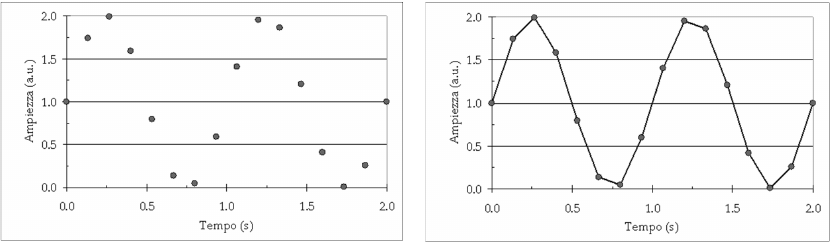
\includegraphics[
        width=8cm,
        height=7cm,
        keepaspectratio,
    ]{images/interpolazioneLineare.png}
    \caption{Un esempio di interpolazione lineare per il campionamento di una sinusoide.}
    \label{interpolazione:lineare}
  \end{center}
\end{figure}
ponendo quindi:
$$
  f_{campionamento} = 2f_{max}
$$
otterremmo un insieme di punti che stanno su una retta parallela all'asse delle ascisse (sul valore $y$ di metà ampiezza del segnale campionato) e, applicando l'interpolazione lineare, andremmo a ricostruire tale retta. Siccome abbiamo campionato una sinusoide, è evidente che l'interpolazione lineare, in questo caso, è stata inefficacie. Come vedremo, in questo caso limte è necessaria l'interpolazione \textit{a seno cardinale}.
\paragraph{Interpolazione polinomiale cubica}~\\
Questo tipo di interpolazione è quello usato da tool come MatLab e Excel per effettuare l'interpolazione. Ricostruisce una curva che passa per i punti sperimentali, mantenendo continue la derivata prima e seconda. Ha quindi l'effetto visivo di una "linea smussata".

La funzione interpolante in questo caso è definita come una funzione che è nulla per tutti i punti appartenenti all'asse $x$ tranne che per i punti dell'intervallo $[-k;k]$ con $k\ \epsilon\ \mathbb{N},\ k  > 1$.
\begin{center}
  E QUA METTICI LA FUNZIONE INTERPOLANTE CUBICA
\end{center}
\paragraph{Interpolazione a seno cardinale}~\\
È il tipo di interpolazione ideale per la ricostruzione di segnali campionati nel tempo. La funzione interpolante è fatta come in Figura \ref{interpolazione:interpolante:seno} ed è possibile ricavarla matematicamente dall'operazione di filtraggio passa-basso ideale del segnale campionato. Nel dominio del tempo consiste in una convoluzione del segnale campionato con la funzione $sinc(\pi x) = \frac{\sin(\pi x)}{\pi x}$, che è continua e non si annulla mai.
\begin{figure}
  \begin{center}
    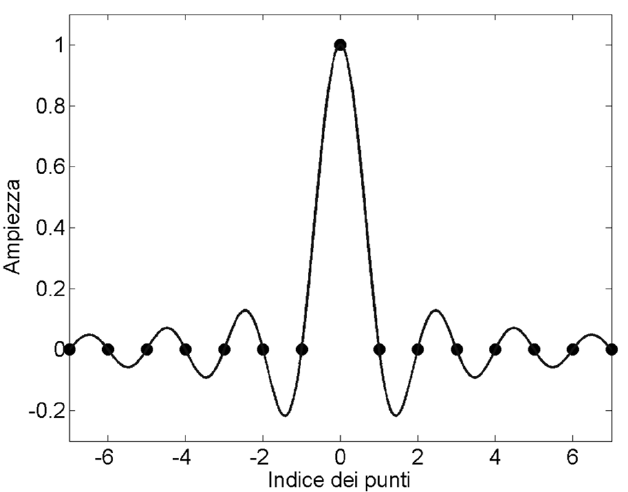
\includegraphics[
        width=8cm,
        height=7cm,
        keepaspectratio,
    ]{images/interpolanteSeno.png}
    \caption{La funzione interpolante a seno cardinale.}
    \label{interpolazione:interpolante:seno}
  \end{center}
\end{figure}
\paragraph{Esempio di ricostruzione di un segnale mediante interpolatore}~\\
In Figura \ref{interpolazione:esempio} possiamo vedere due esempi di interpolazione: una a seno cardinale e una lineare. La differenza che si nota è sostanziale.
\begin{figure}
  \begin{center}
    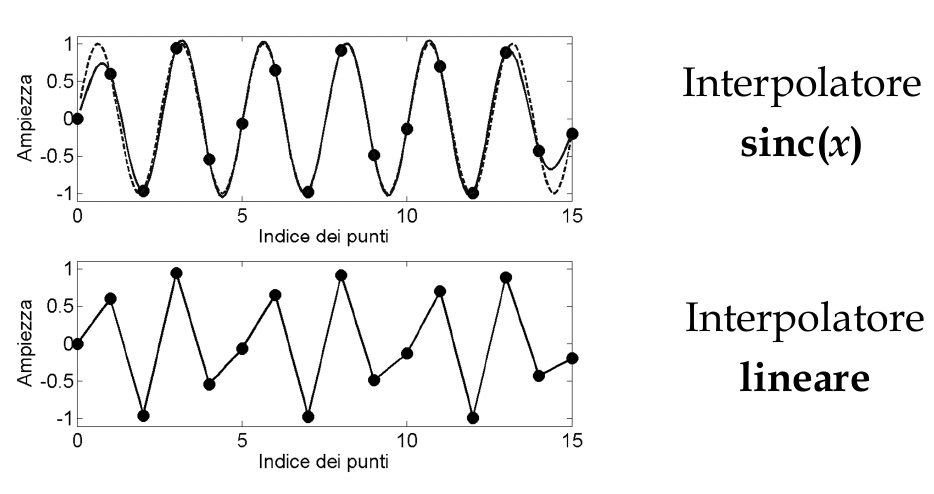
\includegraphics[
        width=8cm,
        height=7cm,
        keepaspectratio,
    ]{images/interpolazioneEsempio.png}
    \caption{Un esempio di interpolazione sia a seno cardinale sia lineare.}
    \label{interpolazione:esempio}
  \end{center}
\end{figure}
Una caratteristica da notare nell'interpolazione a seno cardinale e che si nota dalla Figura \ref{interpolazione:esempio} è la "precisione" dell'interpolazione che diminuisce in prossimità degli estremi dell'intervallo di campionamento, mentre vicino al centro dell'intervallo è molto più "fedele". Questo è dovuto al fatto che tale metodo di interpolazione sfrutta, per determinare un tratto di curva tra due punti sperimentali, l'informazione di tutti gli altri punti sperimentali. In prossimità degli estremi, è quindi impossibile avere informazioi sulle parti "a destra" e "a sinistra", perchè non sono state campionate.
\subsection{Regressione}
\chapter{Esercizi di Conversione}
\section{Conversione di Potenze}
\begin{table}[H]
  \caption{}
  \label{tab:}

  \begin{center}
    \begin{tabular}{|l|r|}
    \hline
    Lineare                 & dB\\
    \hline
       2                    & $\simeq +3$ \\
    \hline
       $\frac{1}{2}$        & $\simeq -3$ \\
    \hline
       $5 = \frac{10}{2}$   & $\simeq +7$ \\
    \hline
       $\frac{1}{5}$        & $\simeq -7$ \\
    \hline
    \end{tabular}
  \end{center}
\end{table}
Per la prima è sufficiente andare a memoria o effettuare un rapido calcolo con la calcolatrice.\\
Per la seconda è necessario usare le proprietà dei logaritmi:
\begin{equation}
  \label{logaritmi:frazione}
  log_{10}(\frac{1}{x}) = log_{10}(x^{-1}) = -log_{10}(x)  
\end{equation}
Per la terza possiamo ancora usare le proprietà dei logaritmi:
\begin{equation}
  \label{logaritmi:differenza}
  10log_{10}(5) = 10log_{10}(\frac{10}{2}) = 10log_{10}(10)-10log_{10}(2) \simeq 10 - 3 = 7  
\end{equation}
mentre per l'ultima si utilizza nuovamente la \ref{logaritmi:frazione}.
\section{Conversione di Ampiezze}
\begin{table}[H]
  \caption{}
  \label{tab:}

  \begin{center}
    \begin{tabular}{|l|r|}
    \hline
    Lineare                               & dB\\
    \hline
       $\sqrt{2}$                         & $\simeq +3$ \\
    \hline
       2                                  & $\simeq +6$ \\
    \hline
       $\frac{\sqrt{2}}{2} \simeq 0.707$  & $\simeq -3$ \\
    \hline
       $5$                                & $\simeq 14$ \\
    \hline
       $\frac{1}{5}$                      & $\simeq -14$ \\
    \hline
    \end{tabular}
  \end{center}
\end{table}
È abbastanza semplice notare come per alcuni valori noti sia sufficiente, se si è già calcolato o se lo si ricorda meglio, raddoppiare il valore in dB della potenza.

Altre operazioni di derivazione (senza calcolatrice o ragionamenti troppo complessi) che possiamo facilmente effettuare sono, per esempio, quelle similari alla prima conversione della tabella. Se conosciamo $10log_{10}(2) = 3$, allora possiamo ricavare facilmente, con le proprietà dei logaritmi:
$$
  20log_{10}(2^{\frac{1}{2}}) = \frac{20}{2}log_{10}(2) = 10log_{10}(2)
$$
Possiamo usare un ragionamento simile a \ref{logaritmi:differenza} per ottenere la terza conversione della tabella: conoscendo la conversione di $\sqrt{2}$ e tenendo presente il fatto che dividere per 2 nel processo di conversione possiamo interpretarlo come sottrarre 6:
$$
  20log_{10}(\frac{\sqrt{2}}{2}) = 20log_{10}(\sqrt{2})-20log_{10}(2) = +3-6 = -3
$$ 
\end{document}
